\documentclass[11pt]{article}

% ---------- Page & typography ----------
\usepackage[a4paper,margin=1in]{geometry}
\usepackage{setspace}
\usepackage{parskip}
\usepackage{microtype}
\usepackage{titlesec}
\usepackage{enumitem}
\usepackage{graphicx}
\usepackage{booktabs}
\usepackage{array}
\usepackage{xcolor}
\usepackage{csquotes}
\usepackage{float}
\usepackage{caption}
\usepackage{subcaption}
\usepackage{fancyhdr}
\usepackage{lastpage}

% ---------- Bibliography first ----------
\usepackage[numbers,sort&compress]{natbib}

% ---------- Links & clever refs ----------
\usepackage[colorlinks=true,linkcolor=black,citecolor=black,urlcolor=blue]{hyperref}
\usepackage[capitalize,nameinlink]{cleveref}

% ---------- Code listings ----------
\usepackage{listings}
\lstdefinestyle{base}{
  basicstyle=\ttfamily\small,
  columns=fullflexible,
  showstringspaces=false,
  breaklines=true,
  frame=single,
  framerule=0.2pt,
  rulecolor=\color{black!15},
  backgroundcolor=\color{black!3},
  captionpos=b,
  xleftmargin=1pt,
  xrightmargin=1pt,
}
\lstdefinestyle{bash}{style=base,language=bash,morekeywords={hadoop,aws,s3,emr,ssh,scp}}
\lstdefinestyle{python}{style=base,language=Python}
\lstdefinestyle{sql}{style=base,language=SQL}

% Convenience environments that behave like lstlisting and accept options
\lstnewenvironment{terminal}[1][]{\lstset{style=bash,#1}}{}
\lstnewenvironment{pycode}[1][]{\lstset{style=python,#1}}{}
\lstnewenvironment{sqlcode}[1][]{\lstset{style=sql,#1}}{}


% ---------- Header / footer ----------
\pagestyle{fancy}
\fancyhf{}
\lhead{Big Data Wrangling with Google Books Ngrams}
\rhead{\thepage\ of \pageref{LastPage}}
\renewcommand{\headrulewidth}{0.4pt}

% ---------- Title block ----------
\title{\vspace{-1.5em}\textbf{Big Data Wrangling With Google Books Ngrams}\\\large Using AWS EMR, HDFS, Spark, and S3}
\author{Ethan Shelburne \\ BrainStation: The Digital Learning Company}
\date{\today}

% ---------- Helper macros ----------
\graphicspath{{figures/}{screenshots/}}
\newcommand{\code}[1]{\texttt{#1}}
\newcommand{\screenshot}[3][0.95]{%
  \begin{figure}[H]
    \centering
    \includegraphics[width=#1\linewidth]{#2}
    \caption{#3}
    \label{fig:#2}
  \end{figure}}

% ---------- Document ----------
\begin{document}
\maketitle
\thispagestyle{fancy}


\tableofcontents
\listoffigures

\newpage



\section{Introduction}

\subsection{Executive Summary}
\label{sec:exec}
This project applies a big–data workflow to the Google Books Ngrams corpus using AWS EMR. We provision an EMR cluster (Spark + HDFS + JupyterHub), connect to the primary node via SSH (and an SSH tunnel for JupyterHub), copy the public CSV from S3 into HDFS, and load it in PySpark. We validate the load (schema, row/column counts, quick ranges), register a temporary view, and run Spark SQL to filter the dataset to the token \texttt{"data"}. The filtered result is written back to HDFS as CSV with \texttt{header=True}, merged to a single local file with \texttt{getmerge}, and uploaded to a personal S3 bucket. Finally, on a local machine we read the S3 object into pandas, save a local copy, and visualize trends over multiple year windows (full range vs.\ consecutive-year subsets), noting peaks in the 1980s/1990s and a decline in the early 2000s. All steps are fully documented with commands and screenshots for reproducibility. Additionally, we compare and contrast Hadoop and Spark in Section \ref{sec:hadoop_et_al}.

\subsection{Dataset Overview}
\label{sec:data_overview}
The analysis uses the English 1-gram slice of Google Books Ngrams. Each row represents a single 1-gram token in a given year with four fields: \texttt{token} (string), \texttt{year} (integer), \texttt{frequency} (total occurrences across all books that year), \texttt{pages} (distinct pages containing the token), and \texttt{books} (distinct volumes containing the token). The series spans from the 1500s through 2008 with sparser coverage in the earlier years. The unfiltered data set includes $261,823,225$ records.




\section{Reproducible Steps \& Command Log}
\label{sec:steps}

\textbf{Note on placeholders.} Replace values in \texttt{<angle brackets>} with your own environment:
\begin{itemize}
  \item SSH key path: \verb|<your_key_path>| (e.g., \verb|/c/Users/you/Desktop/.../key.pem| on Git Bash)
  \item Your S3 bucket/prefix: \verb|s3://<your_bucket>/ngrams/|
\end{itemize}

\subsection{Spin up EMR cluster}
Create an EMR 6.x cluster with Hadoop, Spark, and JupyterHub. Screenshots and specifications are documented in \cref{app:screenshots}.

\subsection{Connect to the head node (SSH)}
\label{ssh}
Open gitbash, and run the following command with the path to your key, and the public DNS of your EMR primary node (which can be copied from your cluster info on AWS under ``Connect to the Primary node using SSH''). This connects you to the head node of your cluster.\\

\begin{terminal} 
ssh -i "<your_key_path>" hadoop@ec2-18-191-151-44.us-east-2.compute.amazonaws.com
\end{terminal}

\subsection{Create HDFS target directory}
Create a target HDFS directory with the following command.\\
\begin{terminal}
hdfs dfs -mkdir -p /user/hadoop/eng_1M_1gram
\end{terminal}

\subsection{Copy public CSV from S3 to HDFS}
Use the following command to copy the the target CSV from the public S3 bucket into the HDFS directory which was just created.\\
\begin{terminal}
hadoop fs -cp s3://brainstation-dsft/eng_1M_1gram.csv hdfs:///user/hadoop/eng_1M_1gram/
\end{terminal}

\subsection{Verify HDFS ingest}

Confirm the CSV file is now in the HDFS directory by listing the directory's contents, then printing the head of the dataset with the following commands.\\

\begin{terminal}
hdfs dfs -ls -h /user/hadoop/eng_1M_1gram
hdfs dfs -cat /user/hadoop/eng_1M_1gram/eng_1M_1gram.csv | head -n 5
\end{terminal}

\subsection{Open a JupyterHub tunnel}
After exiting the previous ssh session, use gitbash to open a tunnel to your primary node with the following command.\\
\begin{terminal}
ssh -i "<your_key_path>" \
    -L 9443:localhost:9443 \
    hadoop@ec2-18-191-151-44.us-east-2.compute.amazonaws.com
\end{terminal}

\noindent In your browser, open \textbf{https://localhost:9443/} and log in with the default credentials (user \texttt{jovyan}, password \texttt{jupyter}). In a PySpark notebook, read the data from 
$$
\verb|hdfs:///user/hadoop/eng_1M_1gram/eng_1M_1gram.csv|,
$$
inspect the structure and schema of the data, filter with \texttt{token=`data'} via Spark SQL, and write the CSV file to $$\verb|hdfs:///user/hadoop/outputs/data_token_csv|$$ with \texttt{header=True}. See all the details of the reading, filtering, and writing process in the notebook \texttt{big\_data\_wrangling\_on\_cluster.ipynb}.

\subsection{Confirm the filtered write in HDFS}

Use the following commands to verify the filtered CSV was successfully written back into HDFS (by checking the directory and printing the head of the data).\\

\begin{terminal}
hdfs dfs -ls -h /user/hadoop/outputs
hdfs dfs -cat /user/hadoop/outputs/data_token_csv/part-*.csv | head -n 10
\end{terminal}

\subsection{Merge to a single local CSV on the head node}

Next, use the following commands to collect the contents of \texttt{data\_token\_csv} into a single file on the local drive of the head node.\\

\begin{terminal}
# Create a local folder
mkdir -p ~/ngrams_outputs

# Merge the directory into one local file
hdfs dfs -getmerge /user/hadoop/outputs/data_token_csv/ ~/ngrams_outputs/data_token.csv

# Confirm data was correctly copied to the local drive of the head node
head -n 5 ~/ngrams_outputs/data_token.csv
\end{terminal}

\subsection{Upload merged CSV to your S3 bucket}

Move the CSV file from the local drive of the head node into a S3 bucket in your account using the following commands.\\

\begin{terminal}
# Upload the CSV to your S3 bucket
aws s3 cp ~/ngrams_outputs/data_token.csv  s3://<your_bucket>/ngrams/data_token.csv

# Verify it now exists in your bucket
aws s3 ls s3://<your_bucket>/ngrams/
\end{terminal}
Once, the file has been successfully copied into your bucket, terminate your cluster.

\subsection{Local machine: load \& plot with pandas}
The following commands configure your local AWS CLI credentials and install the Python package needed to read data into pandas from S3 buckets.\\

\begin{terminal}
# Configure AWS CLI credentials 
aws configure
#   AWS Access Key ID: <your_access_key_id>
#   AWS Secret Access Key: <your_secret_access_key>
#   Default region name:   us-east-2 
#   Default output format: json

# Install required packages for local analysis
pip install s3fs
\end{terminal}

Next, load the CSV from your S3 bucket and produce the plots in your local notebook; see the notebook \texttt{big\_data\_wrangling\_on\_local.ipynb} for the full code and outputs.



\section{Hadoop, HDFS, and Spark}
\label{sec:hadoop_et_al}

\subsection{Hadoop vs.\ Spark}
\label{sec:hadoop_spark}


Hadoop MapReduce expresses jobs as a sequence of map and reduce phases. Each phase writes intermediate results to disk, which makes it robust but incurs significant resource cost for iterative workloads. Spark uses a DAG (Directed Acyclic Graph) scheduler over Resilient Distributed Datasets (RDDs), which are immutable, partitioned collections of records that enable fault-tolerant parallel operations. Stages are pipelined, and intermediate results are cached in memory (spilling to disk as needed). This design dramatically reduces repeated disk load and lowers end-to-end cost for many workloads.


Both run at cluster scale and integrate with HDFS, S3, and YARN. Hadoop MapReduce remains strong for very large batch ETL where jobs are straightforward and fault tolerance via re-execution is acceptable. Spark is preferred for iterative algorithms (machine learning, network science, queries with many joins), ad-hoc analysis, streaming, and interactive notebooks.

\paragraph{Two advantages of Hadoop (MapReduce).}
\begin{itemize}
  \item \textbf{Simplicity and durability for batch.} The disk-centric map/reduce stages are simple, restartable, and well-suited to massive ETL.
  \item \textbf{Mature integration with HDFS/YARN.} Decades of operational experience, strong data locality with HDFS, and a broad set of Hadoop ecosystem tools.
\end{itemize}

\paragraph{Two advantages of Spark.}
\begin{itemize}
  \item \textbf{Performance for iterative/interactive jobs.} In-memory caching and a DAG optimizer expedites iterative jobs (like machine learning algorithms) compared to the disk-bound MapReduce.
  \item \textbf{Unified high-level APIs.} Spark DataFrames/Spark SQL, MLlib, and Structured Streaming provide a single programming model across batch, SQL, ML, streaming, and other big data tasks.
\end{itemize}

\subsection{HDFS as a Storage System}
\label{sec:hdfs_storage}

HDFS stores files by splitting them into large fixed-size blocks (128~MB by default in Hadoop 3). Each block is replicated across multiple DataNodes (default replication factor is 3). A central \textbf{NameNode} maintains the filesystem namespace and block metadata (which blocks belong to which file, and where those blocks live), while \textbf{DataNodes} store the actual block bytes.

To create a file, a client asks the NameNode to allocate a path and block targets. The client then streams data to a replication pipeline of DataNodes; acknowledgements flow back up the pipeline only after each packet is written to each replica. HDFS follows a single-writer, multiple-reader model with write-once (append-supported) semantics, which simplifies consistency and recovery. For reads, the client requests block locations from the NameNode and then fetches the closest replica. This design exploits data locality: compute tasks are scheduled where the data already resides to reduce network expense. DataNodes send block reports to the NameNode. If a DataNode fails or a replica falls below the target replication factor, HDFS automatically re-replicates blocks to healthy nodes. Tools such as the balancer help maintain even distribution and detect inconsistencies. 

In summary, HDFS is a distributed filesystem designed to live inside the compute cluster. That tight coupling enables locality-aware scheduling and high throughput for large sequential reads and writes.



\appendix

\section{Screenshots for Cluster Setup}
\label{app:screenshots}
\appendix

Spin up an EMR cluster with emr-6.10.0 and the following custom application bundle.

\begin{figure}[H]
  \centering
  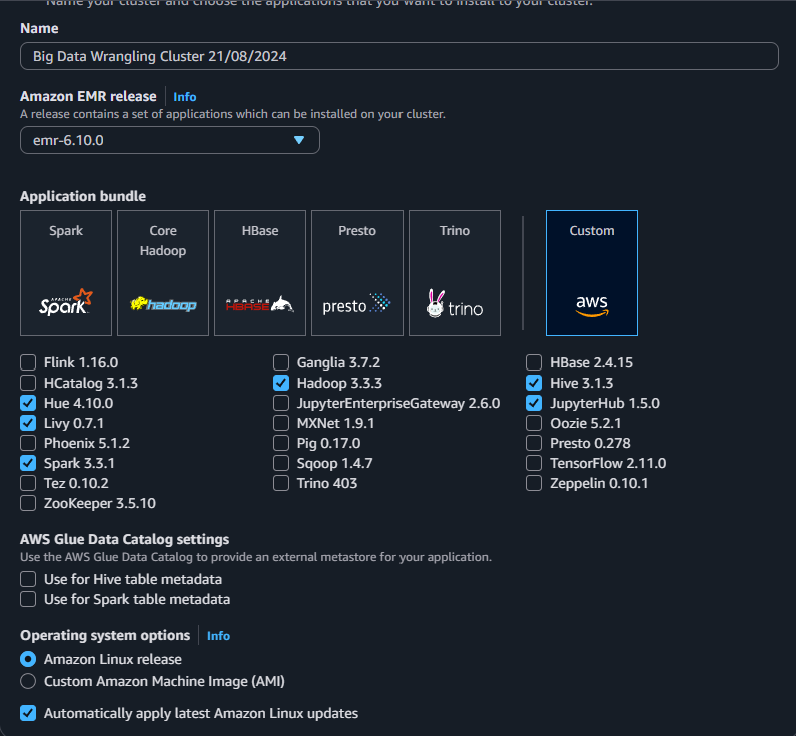
\includegraphics[width=.7\linewidth]{SCREENSHOTS/cluster_set_up_1.png}
  \caption{Custom application bundle}
  \label{fig:cluster-setup-1}
\end{figure}

Remove the ``Task'' instance group and set the other instance groups (``Primary'' and ``Core'') to \texttt{m5.xlarge} types. 

\begin{figure}[H]
  \centering
  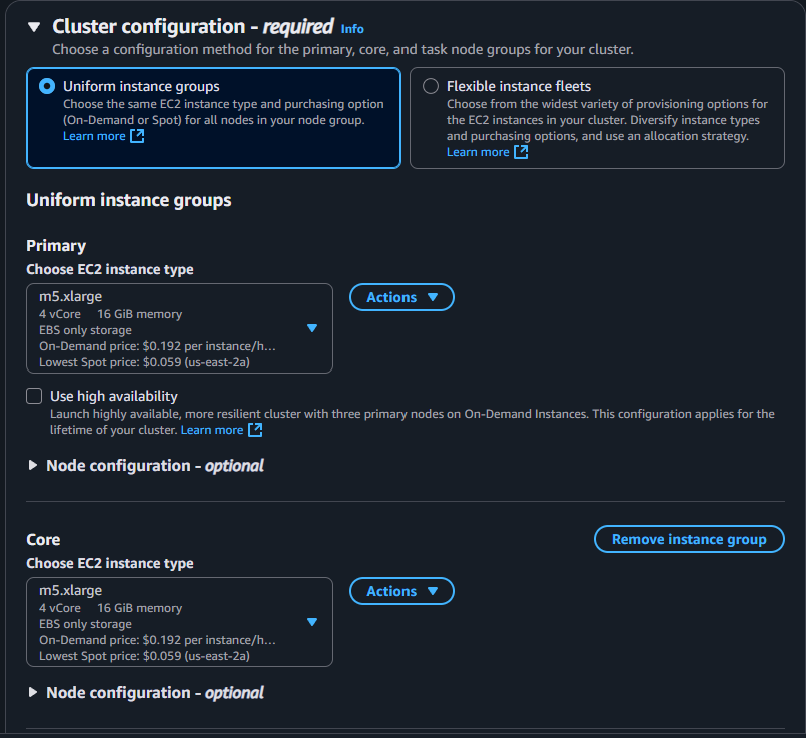
\includegraphics[width=.7\linewidth]{SCREENSHOTS/cluster_set_up_2.png}
  \caption{Configure uniform instance groups}
  \label{fig:cluster-setup-2}
\end{figure}

Set the cluster size manually so that the ``Core'' instance count is $2$.

\begin{figure}[H]
  \centering
  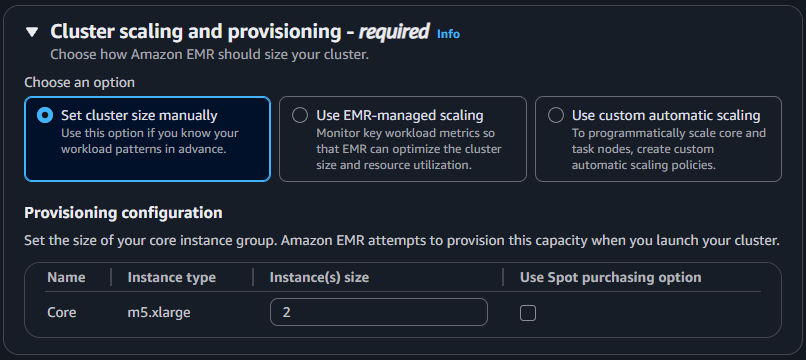
\includegraphics[width=.7\linewidth]{SCREENSHOTS/cluster_set_up_3.png}
  \caption{Set ``Core'' instance count to $2$}
  \label{fig:cluster-setup-3}
\end{figure}

Set auto-termination after 2 days of idle time. We chose to set this metric to 2 days to ensure the cluster would not be accidentally terminated (which could lead to lost work). The steps in Section \ref{sec:steps} should take much less time than this so it is essential to manually terminate the cluster when all steps are complete. 

\begin{figure}[H]
  \centering
  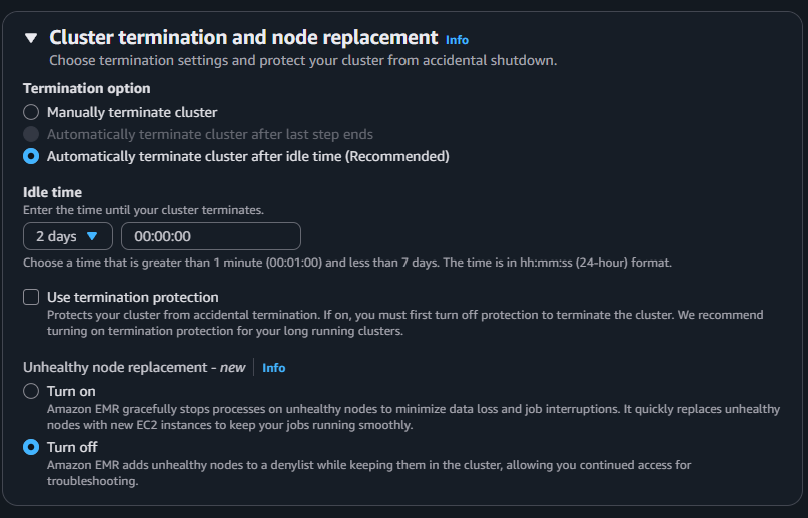
\includegraphics[width=.7\linewidth]{SCREENSHOTS/cluster_set_up_4.png}
  \caption{Specify cluster termination options}
  \label{fig:cluster-setup-4}
\end{figure}

Under the security configuration settings, select your EC2 key pair (ensuring you are in the correct AWS geography). The path to this key pair will be used throughout Section \ref{sec:steps}.

\begin{figure}[H]
  \centering
  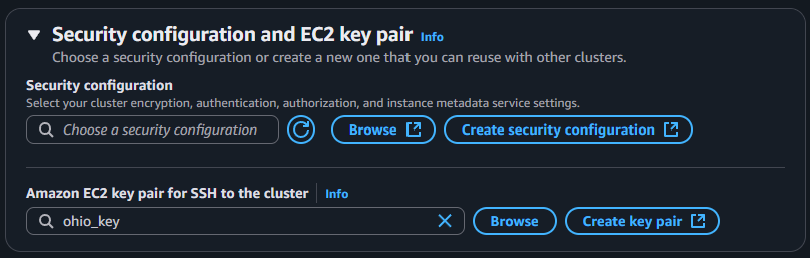
\includegraphics[width=.7\linewidth]{SCREENSHOTS/cluster_set_up_5.png}
  \caption{Select EC2 key pair}
  \label{fig:cluster-setup-5}
\end{figure}

In the ``Identity and Access Management'' section, select \texttt{EMR\_DefaultRole} and \texttt{EMR\_EC2\_DefaultRole} under ``Amazon EMR service role'' and ``EC2 instance profile for Amazon EMR'' respecitvely.

\begin{figure}[H]
  \centering
  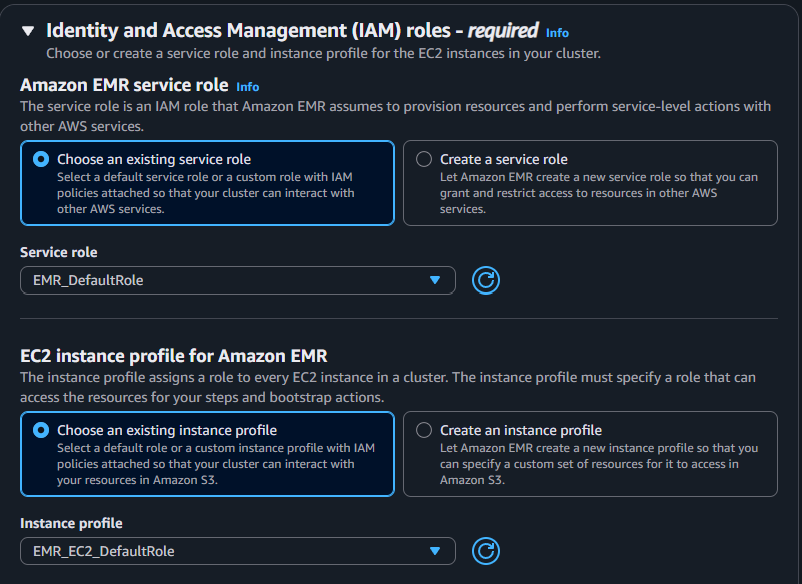
\includegraphics[width=.75\linewidth]{SCREENSHOTS/cluster_set_up_6.png}
  \caption{Configure IAM Roles}
  \label{fig:cluster-setup-6}
\end{figure}


Click on ``Create cluster'' to finish the set up. When provisioning is finished and the EMR instance is ready, the cluster state should be ``Waiting.'' At this point, run the command from Section \ref{ssh} in GitBash to connect to the head node of the cluster and get the following message.

\begin{figure}[H]
  \centering
  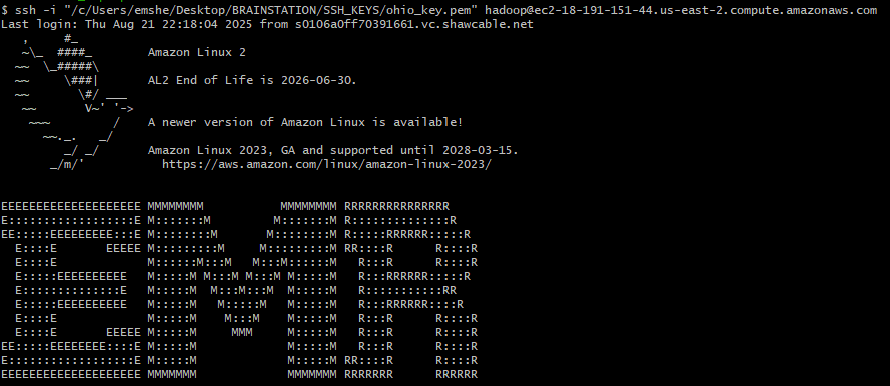
\includegraphics[width=.75\linewidth]{SCREENSHOTS/ssh_to_cluster_screenshot.png}
  \caption{SSH to primary node}
  \label{fig:ssh-primary}
\end{figure}




\end{document}